%
% geodesics.tex
%
% (c) 2024 Prof Dr Andreas Müller
%
\begin{figure}
\centering
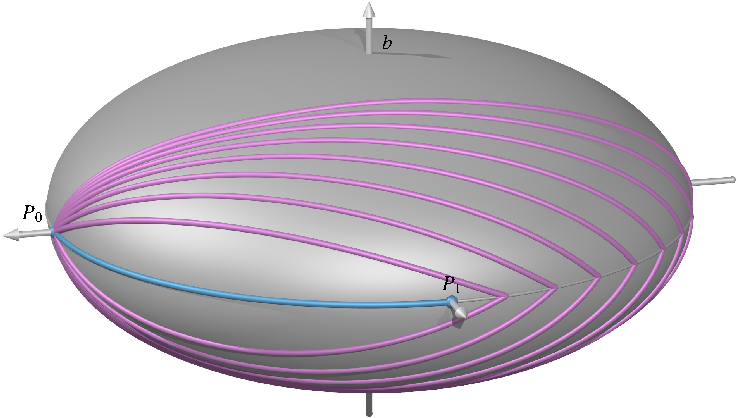
\includegraphics{chapters/060-variation2/examples/geodesics.pdf}
\caption{vom Punkt $P_0$ ausgehende Geodäten auf einem Rotationsellipsoid
mit Äquatorradius $1$ und Polradius $b$.
Die Kurve entlang des Äquators (blau) ist eine Lösung der
Euler-Lagrange-Differentialgleichung und sie erfüllt immer die starke
Legendre-Bedingung, aber das Jacobi-Kriterium ist nicht erfüllt, wenn 
sie länger als $b\pi$ wird.
Bei dieser Länge findet man den konjugierten Punkt $P_1$, ab
dieser Länge sind die rosaroten Geodäten kürzer.
\label{buch:variation2:fig:geodaeten}}
\end{figure}
